% !TEX TS-program = xelatex
% !TEX encoding = UTF-8 Unicode
\documentclass{article}
% \usepackage[utf8]{inputenc}
\usepackage[margin=3cm]{geometry}
\usepackage{fontspec}
\setmonofont[Scale=0.7]{Monaco}
\usepackage[backend=biber, sorting=nty, doi=false, style=verbose]{biblatex}
\addbibresource{./examen.bib}
\usepackage{hyperref}
\usepackage{afterpage}
\usepackage{pdfpages}
\usepackage{graphicx}
\usepackage{caption}
\usepackage{subcaption}
\usepackage{listings}
\usepackage[T1]{fontenc}
\usepackage{csquotes}
\usepackage{relsize,etoolbox}% http://ctan.org/pkg/{relsize,etoolbox}
\usepackage[swedish]{babel}
% \usepackage[T2A]{fontenc}
\graphicspath{ {./img/} }
\newcommand\blankpage{%
	\null
	\thispagestyle{empty}%
	\newpage
}
\captionsetup{justification=raggedleft,singlelinecheck=false}
\renewcommand{\baselinestretch}{1.5}
\lstset{basicstyle=\ttfamily\footnotesize, tabsize=2} \usepackage[framed, numbered]{sclang-prettifier}
\interfootnotelinepenalty=10000
\AtBeginEnvironment{quote}{\smaller}% Step font down one size relative to current font.

%%%%% Kompilera med xelatex!!!!! %%%%%


%\title{%
%	%Liminal Space - An Aesthetic \\
%	%Gränslandets estetik \\
%   Gränsland
%	\large{Vad har utommusikaliska referenser för roll i det elektroakustiska komponerandet?}
%}
%\author{Viktor Sandström}
% \date{Februari 2022}


\begin{document}
% \maketitle
\begin{titlepage}
	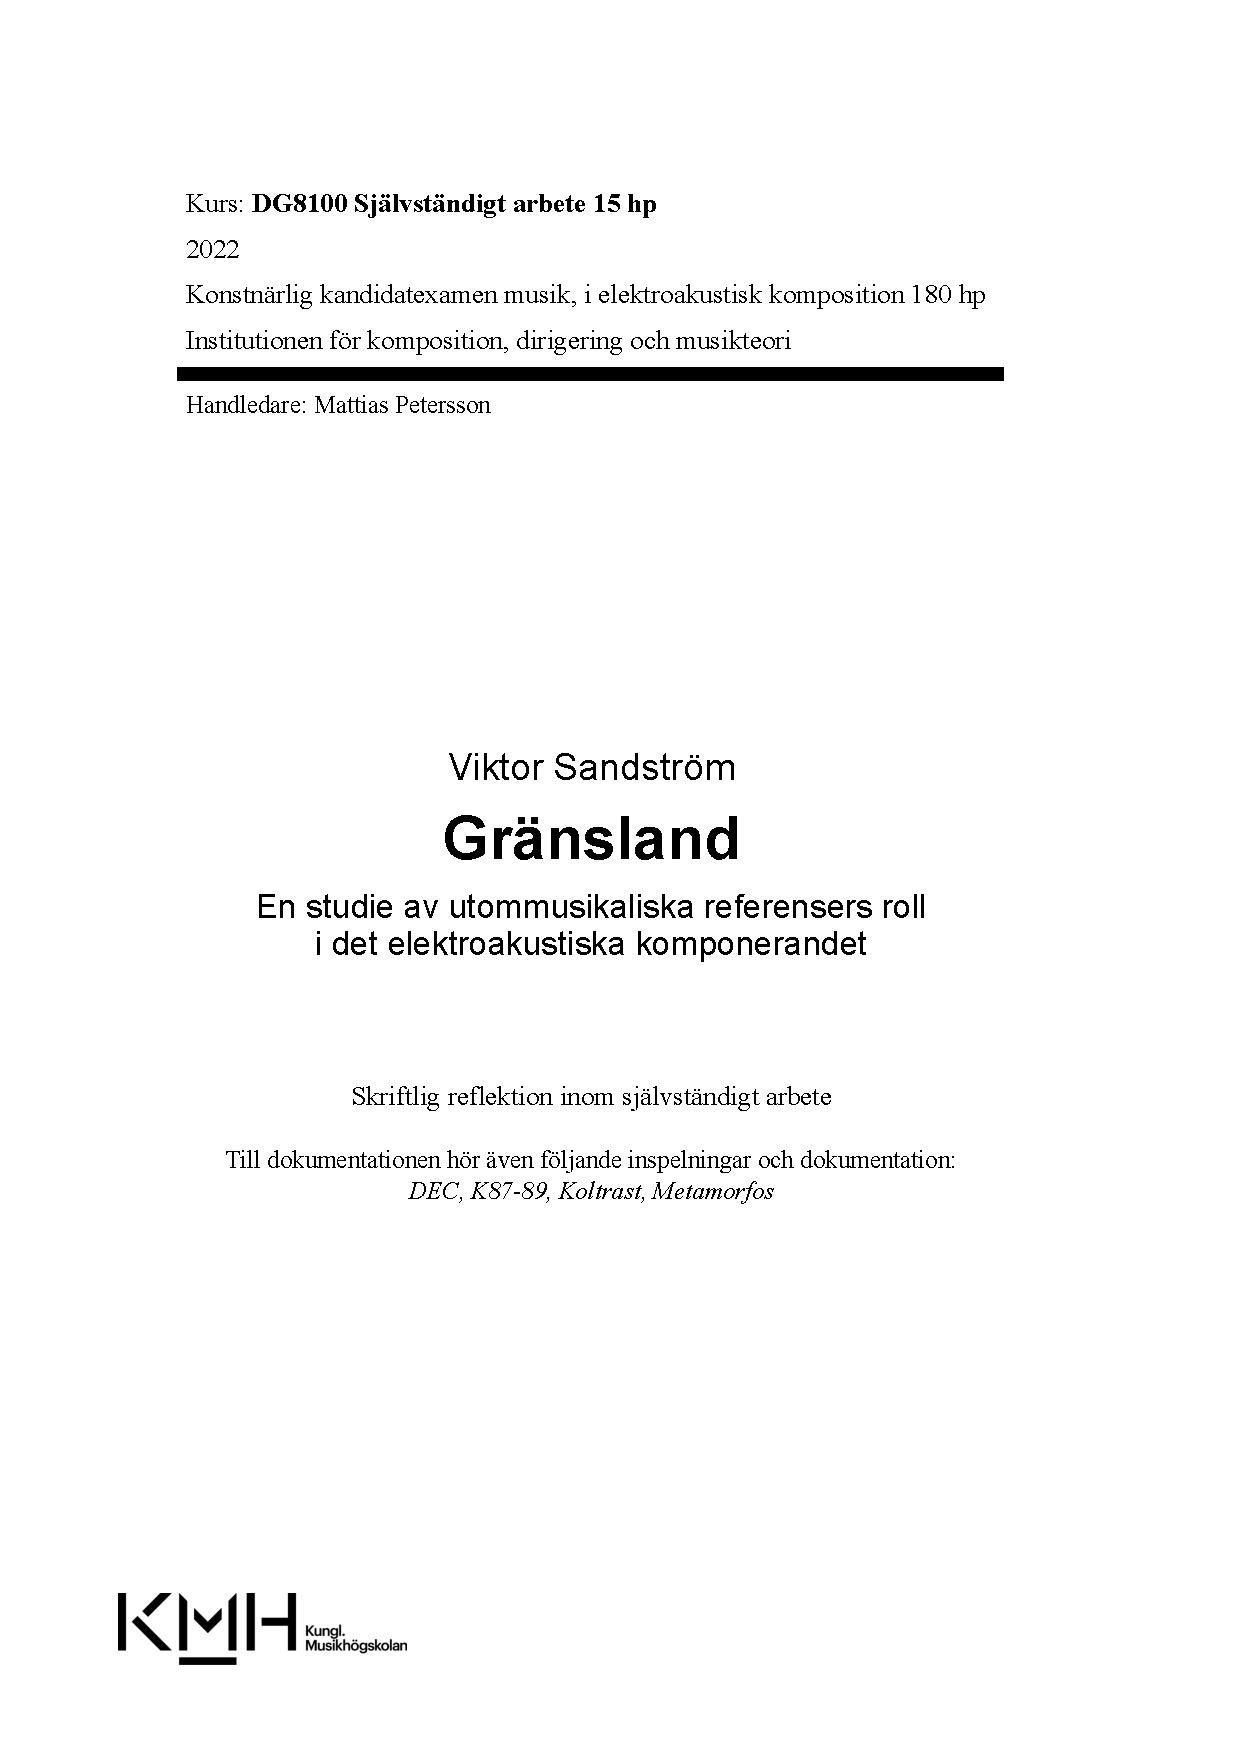
\includepdf[pages={1-2}]{./Framsidauppsats.pdf}
\end{titlepage}

\begin{center}
	\hspace{0pt}
	\vfill
	\emph{Any sufficiently advanced technology is indistinguishable from magic\footcite{ArthurCClarkeMagic}}
	\vfill
	\hspace{0pt}
\end{center}
\newpage
\tableofcontents
\newpage

\section{Inledning}
% ny inledning:
Under åren 2020-2021 genomgick jag en lång sjukskrivning. Jag spenderade större delen av den här perioden i
mitt hem, med undantag för sjukhusbesök, ett julfirande och min trettioårsdag. Under den här sjukdomstiden
började jag skriva musik, mest ur en frustration av att plötsligt ha så mycket tid, något som jag
tidigare klagat över att jag inte hade haft. Eftersom min vardag bestod utav repetition var min impuls att
skriva om det jag såg. Jag hade fattat tycke för de märkliga, bortglömda miljöerna som finns på sjukhus och
vårdmottagningar, som existerade mitt i en plats som aldrig sov, som ständigt var i rörelse, men där miljöerna
själva såg obefolkade och stillastående ut, som att deras funktionalitet hade gått förlorad. En sådan typ av
plats som jag reagerade starkt på var de innergårdar, som var anlagda med promenadstråk, välskötta buskar
och träd och små konstellationer av parkmöbler övervuxna med alger som låg insprängda mellan
sjukhusbyggnaderna. Eller de oändligt långa korridorerna i sjukhuset, tomma på människor, med dammig och
bortglömd offentlig konst. 
%Gjorde om lite här. får se om det känns som att det är bra
Min ursprungliga idé var att använda de här miljöerna i ett kompositionsarbete. 
Miljöerna kändes stillaståeende och tidlösa och jag fann att de på ett sätt speglade min egen tillvaro. Idén
övergick gradvis till att handla om att dokumentera min egen stillastående vardag.

% När jag började må bättre ...
När jag började må bättre fann jag att det inte hade varit tid utan ork jag hade saknat tidigare, och det var
först då som jag hade orken att arbeta med den här idén. I och med en förbättring av
mitt mående och ett överskott av ledig tid kunde jag ta mig an att lära mig programmeringsspråket 
SuperCollider\footcite{sc}, ett språk utvecklat för ljudbehandling och
komposition, ett verktyg som jag tidigare önskat lära mig men inte orkat. I och med detta och ett ökat
intresse för datorprogrammering i allmänhet föll det sig naturligt att mycket av musiken jag skrev blev
skriven med hjälp av detta verktyget.

Under min utbildning har det ofta känts som att jag jagat ett ideal av vad elektroakustisk konstmusik är. En
känsla av att inte hinna lära sig alla tekniker som är aktuella inom det elektroakustiska fältet, och att
ständigt göra musik som på ett eller annat sätt är en del av en lärandeprocess, men som är påeldad av
prestationsångest och en känsla av att inte veta vad man gör. En insikt var att mycket, om inte allt jag gjort
under åren varit något likt en \emph{tech-demo}, ett ljudande exempel på vad en teknik kan erbjuda, utan att jag
haft en känslomässig förankring i materialet.

% Också omformulerad, förhoppningsvis tydligare
Jag använde en kompositionsmetod som kändes annorlunda från hur jag tidigare arbetat, och i relation till min
erfarenhet av att skriva musik inom utbildningens kontext. 
% 
Musiken var inte längre ett medel för att uppnå målet att bemästra en ny teknik. Istället fanns en känsla av
att kunna få utforska tekniken om ett behov fanns, eller av nyfikenhet, men där ett estetiskt uttryck fick
vara förgrund för processen.
% Kan bli en bra slutkläm, men förtydliga för att få till det
Jag blev också intresserad av att undersöka hur detta estetiska uttryck skulle kunna förmedlas. Kan åhöraren
förnimma ett narrativ, eller vad är det som förmedlas genom musiken? Är det möjligt att en filtrerad version,
frånkopplad från kompositörens landskap av associationer och referenser, skulle kunna förmedla något som ändå
liknade dess källa? Att lyssnaren kunde förnimma gestalten av ett sånt landskap, men inte innehållet.



% ////////
\pagebreak
\section{Bakgrund}
% Flytta till Bakgrund

I François Delalandes uppsats "Music Analysis and Reception Behaviours: Sommeil by Pierre Henry"
\footcite[26, 38, 52]{Delalande1998} presenterar han tre typer av lyssnarbeteenden, eller analysmetoder, det
\emph{taxonomiska}, det \emph{empatiska} och det \emph{figurativiserande}. Det \emph{taxonomiska} påminner om
traditionell musikanalys, att försöka strukturera och klassificera ljud längs en tidslinje. Det
\emph{empatiska} intresserar sig för de känslointryck som musiken ger lyssnaren i stunden, utan att tänka så mycket på
form. Det \emph{figurativiserande} lyssnar med ett perspektiv som tillåts associera fritt kring de
ljud den hör och använda ljuden som scener som beskriver ett narrativ. Lyssnaren förnimmer narrativet eller
scenen genom musiken. De grupperar liknande ljud, men motsatt till det \emph{taxonomiska}, kopplas ljudet till
en entitet, ett ting eller något levande, och tolkas som rörelse istället för en serie diskreta händelser. Jag
kommer senare i texten utgå från det figurativa lyssnadet för att diskutera generativa metoder som arbetar med
utommusikaliska associationer. 

% Utveckla och bind över till tekniken.

\subsection{Elektronisk musik och teknologi}
Elektrakustiska kompositörer har alltid varit intresserat av, och haft ett intimt förhållande till teknologi.
Utan nya upptäckter under 1800-talet och vidare under 1900-talet hade elektronisk musik, som vi hör den idag,
inte varit möjlig. Uppfinningar som radion, trådlös och trådburen elektrisk signal, magnetband, mikrofoner,
datorer och dess språk samt digital signalprocessering\footcite[1-5]{dsp} etc, har på ett eller annat sätt
möjliggjort och utvecklat musiken. Studion som instrument har alltid varit central inom elektronisk musik,
idag mer än någonsin, med det ständigt sjunkande priset av en persondator, som en produkt av en
kapplöpning mellan ``Moore's law''\footnote{Moore's Law, en av grundarna för Intel som hävdar att processorer
kommer dubbla sin kapacitet varannat år.}, processeringsförmåga och nya billigare tillverkningsmetoder. Idag
kan en produktionsstudio för hemmabruk rymmas i en dator som ryms på ett enda kretskort, som Raspberry
Pi\footcite{rpi}, med ett pris som ligger mellan 150 - 350kr. Tillgängligheten till en studio, som tidigare
var begränsad till institutioner som nationella radiostationer, har gradvis hamnat inom räckhåll för
individen.

% Demokratiseringen av studion.
I och med att denna teknik förflyttats närmare individen har den demokratiserats. Musikteknik har i teorin
aldrig varit så tillgängligt. Dessa hjälpmedel för att skriva, spela in och producera kan rymmas i
fickan på sin användare.

% Bygg ut, vad finns det för några hjälpmedel / verktyg idag? Garageband etc
Trots denna tillgänglighet finns det fortfarande barriärer. Hinder i form av svårtillgänglig information,
eller avskräckande konfigurationssteg som förutsätter en hög grad av förkunskap för att du ska kunna få
tillgång till funktionaliteten du egentligen vill komma åt. Den tidigare nämnda Raspberry Pi-mikrodatorn
stämmer in på den beskrivningen, som trots sitt överkomliga pris förutsätter att du är bekväm att lämna
etablerade operativsystemsparadigmer som Windows och MacOS, kunna utföra kommandon i en
shell-miljö\footcite{unix}, och kunna felsöka när installationer eller konfigurationer inte genomförs
eftersom dessa kommandon kan vara mycket obskyra för den oinvigde.
	
På detta vis är vi också fast i en marknad där dessa open source-verktyg drunknar på grund av sin egen
otillgänglighet, verktyg\footnote{Jag använder termen \emph{verktyg} för att prata om musikutrustning och
teknologier i en bred bemärkelse, från hårdvara till mjukvara} som annars skulle kunna öppna dörrar för många
till experimentell, algoritmisk elektronisk musik, och musikproduktion i stort. Denna marknad består av
musikteknologi som säljs för höga summor, något som med open source-teknologi skulle kunna vara mycket lätt
att ersätta, men som marknadsförs till oss som en \emph{easy fix}, något som inte bara underlättar och
överbryggar tröskeln till det tekniska, men också till det estetiska. Dessa verktyg säljs med idén att om du
bara behöver skaffa dig en sista pryl kommer kreativiteten att flöda. Tidigare banbrytade verktygstillverkare,
som Moog, eller Dave Smith Instruments, säljer nu sina instrument som high-end-utrustning. De är brukbara och
låter väldigt bra, men de är så dyra att priset stänger dörren för den som som försöker ge sig in i musiken,
eller är demoraliserande för den som tänker att verktyget kommer lösa dess problem. De är otillgängliga
ekonomiskt men ur ett popkulturellt perspektiv mycket tillgängliga, eftersom populära verktyg blir synonyma
med ett ljud, en stil, en kultur och med musikalisk och ekonomisk framgång. Ett exempel på detta är den
legendariska TB303\footcite{303}-synten från Roland, som genom sitt stilbildande ljud, känt genom
Detroit-techno, idag är synonymt med elektronisk dansmusik, som idag säljs för mellan 2 -- 5 gånger sitt
säljpris från år 1982\footnote{Originalpris: \$395.00 . Efter inflationskompensation: \$1,161.32. På Ebay
2022: \$5,543.64}. Ett begrepp som används för att beskriva detta fenomen är \emph{G.A.S} - \emph{Gear
acquisision syndrome}\footcite{gas} (eller på svenska \emph{utrustningsanskaffningssyndrom}). Den som drabbas
av detta har fullständigt accepterat det narrativ som sälj till en.
% Fenomenet \emph{G.A.S.} - \emph{Gear acquisision syndrome}\footcite{gas} (eller på svenska \emph{utrustningsanskaffningssyndrom}), innebär i praktiken att man fullständigt
% accepterat det narrativ som säljs till en. 
Om ett företag säljer ett nytt verktyg, med en effektiv marknadsföring bakom sig, kommer forum och trådar på
sociala medier fyllas med ivriga entusiaster som proklamerar att de \emph{``behöver detta!''}. Inom marknaden
för hårdvara, som synthar och studioutrustning är det här en stark köpargrupp och på grund av detta utvecklas
och säljs en stor mängd verktyg som enbart är kopior av tidigare erkända verktyg. Ett tydligt exempel på detta
är Behringer, som till synes baserat sin affärsmodell på kraften hos \emph{G.A.S.}, då de släpper kopior av
instrument som tidigare varit ouppnåeliga, och gör det på så sätt möjligt för många med
\emph{utrustningsanskaffningssyndrom} att ``anskaffa'' den utrustning de känt att de saknat.


Inom elektroakustisk musik kan snarare en motsatt reaktion uppstå. Här ges de mer obskyra verktygen spelrum,
och blir i sig en statussymbol i sin otillgänglighet. De tidigare nämnda verktygen som är svåra för den
vanliga brukaren av musikteknologi blir här ett verktyg för att visa sin virtuositet. Istället för att använda
färdiga verktyg för att åstadkomma ljud, och applicera sin kunskap om olika syntesmetoder på en mjuk- eller
hårdvarusynt, kan du nu skriva ljudprocesseringsalgoritmer själv och på egen hand hushålla med din dators
resurser. Här kan \emph{G.A.S.} yttra sig annorlunda, framförallt inom utbildningar i elektroakustisk
musik. Visserligen möjliggör sådan teknik större flexibilitet och en inspirationkälla i att utforska tidigare
onåbara delar av ett ljudprogram, icke-linjära strukturer av musik och möjligheten att påverka ljud i ett
``close to the metal''-perspektiv, bearbetningar av dess data och form nere på en processorcykelnivå. Dock kan
detta bli till en fälla, då man istället för att använda färdigbyggda verktyg som hjälpmedel, envisas med att
göra det själv.

% La Meme Young
I podcasten \emph{La Meme Young}\footcite{LaMemeYoung} har kompositörerna Max Alper och Jessica Ekomane ett
samtal om att fastna för mycket i den tekniska aspekten av elektronisk konstmusik. De beskriver ett scenario
där en student på masternivå arbetar under hela sin studietid med att bygga sitt verktyg, sitt instrument,
förfinar alla aspekter och reder ut alla buggar och grafiska fulheter, för att sedan avsluta utbildningen utan
att ha skrivit musiken det här instrumentet skulle hjälpa till med att skriva. Hur instrumentet i sig blivit
så omfattande och invecklat att det är svåröverskådligt hur ett komponerande med det ens skulle se ut. Joanna
Demers skriver i \emph{Listening Through The Noise}: ``The sheer freedom of electroacoustic music constitutes
both its strength and its burden.''\footcite{JoannaDemers} Joanna Demers pratar om den oslagbara friheten hos
elektronisk musik. Klangvärlden hos elektronisk musik har till synes oändlig potential.
% bytte ut det följande från ", som trots vad detta utlovar kan vara till dess nackdel."
Denna frihet kan dock bli en nackdel för den elektroakustiska kompositören. I Linus Hillborgs uppsats
\emph{Återbruk och återgivning}\footcite{LinusHillborg} skriver han om teknologiers begränsingar, hur det
kreativa kan komma ur möjligheternas begränsning. Genom att utforska var den gränsen går kan man även hitta de
särskiljande kvalitéer som möjliggör något som är unikt för den teknologin. Det kreativa arbetet kan då likas
vid att känna sig fram i blindo längs en ojämn yta för att lokalisera och kartlägga det intressanta, samt att
lyfta fram det i ljuset.

% Donna Haraway - Cybernetic Manifesto

% Brian Eno - studion som instrument. 

\subsection{Absolut musik och programmusik.}
Demers diskuterar hur man som elektroakustisk kompositör kan förhålla sig till utommusikaliska referenser.
Hon hävdar att inom konservatorier har \emph{absolut musik} historiskt sett fått störst spelrum och har ansetts
som norm. Det är en modernistisk stil som speglar den modernistiska synen på objektivitet, där musiken eller
konsten ska stå för sig själv som något sant och fullkomligt. Likaså är den absoluta musiken en musik vars
mening och syfte är sprunget ur dess egen fullkomlighet, istället för att hänvisa eller berätta om något
utommusikaliskt \footnote{\emph{Extramusical}. Med utommusikaliskt menas något som ligger utanför musiken,
``lying outside the province of music'', strikt tolkat allt som inte innefattas inom det fysikaliska i
ljudvågor som sammanfaller i luften, eller som innefattas inom de regler för ljud-, form- och harmonilära
används för att beskriva musik. \\ Merriam-Webster [Uppslagsverk],
\url{https://www.merriam-webster.com/dictionary/extramusical} (hämtad 2022-03-29)}\nocite{webster}

Ofta benämns motsatsen till den \emph{absoluta musiken} som \emph{programmusik}. Det härstammar från när
kompositörer skrev musik som ville gestalta något utommusikaliskt, där musiken var det bärande berättande
elementet, där programbladet på en sådan konsert var en viktig bilaga för att förstå handlingen i musiken.
Ett exempel på detta är verket \emph{Tavlor på en utställning}\footcite{Tavlor} av Modest Musorgskij,
där varje sats motsvarar en tavla på en utställning, där tavlornas motiv blir levande i musiken. Förklaringar
och målande beskrivningar finns att läsa om varje sats i ett programblad för publiken att orientera sig.

Demers frågar sig var den elektroakustiska musiken platsar in mellan dessa två motstridiga begrepp och
benämner två kompositörer som har varit viktiga för teoretiserandet kring elektroakustisk musik, Pierre
Schaeffer\footcite{PierreSchaeffer} och Trevor Wishart\footcite{TrevorWishart}. Hon menar även att den
elektroakustiska musiken har andra förutsättningar än traditionell, akustisk musik på grund utav dess
ljudmässiga frihet och frågar sig vad det innebär för dess associativa förmåga. ``Are sounds always
referential? Is it possible to hear sound before it has been laden with the associations of culture, history,
or society?''.\footcite[23]{JoannaDemers} Kan de ljud som frammanas inom elektroakustisk och akusmatisk musik
existera utanför sig själva? Kan de vara självrefererande, eller kan de existera, likt Pierre Schaeffers teori
om ljudobjekt \footcite[271]{PierreSchaeffer}, som ljud där ursprunget inte längre är urskiljbart?

Begreppet akusmatisk härstammar från Pythagoras\footcite{oxford} och betyder ljudande men osedd. Han använde
sig av ett skynke under föreläsningar för att att de som lyssnade skulle vara frånskilda talaren, liksom
akusmatisk musik använder sig av högtalaren för att vara frånskilda ljudkällan. Det har inom den
elektroakustiska traditionen använts för att beskriva de teorier Schaeffer lade fram kring att analysera och
tolka ljud utan att se objektet som skapar ljudet. Det ska då gå att tolka ljudet utifrån dess texturer och
kvalitéer snarare än dess förmåga att berätta något om dess källa. Schaeffer myntade uttrycket \emph{reducerat
lyssnande} för att beskriva denna analysmetod, som ska göra lyssnaren fri från ljudets inbyggda associationer.
Istället ska man höra ljudet som det existerar i sin mest avskalade, \emph{sanna} form. Demers ställer
Schaeffers teori kring ljudobjekt mot Trevor Wisharts omtolkning av begreppet; ``Wishart feels that it is
impossible to separate sounds from their associations, so it is incumbent upon the composer to acknowledge and
work with sound references rather than repress them''. Wishart utveckar detta i \emph{On Sonic
Art}\footcite{TrevorWishart} där han ställer sig skeptisk till Schaeffers reducerade lyssnade, och menar att
ljud aldrig kan vara frånskilda en association. Han använder sig istället av begrepp som reella och
icke-reella ljud, reella och icke-reella rum samt något som han benämner som imaginärt/surrealistiskt för att
prata om musik som landskap\footcite[144-147]{TrevorWishart}. Han menar att reella är de ljud som är naturligt
förekommande (röst, traditionella musikinstrument eller naturen etc.), och icke-reella är de från en
onaturlig, konstgjord källa (ett elektroniskt bearbetat ljud eller synthesizer etc). De kan sedan placeras i
en naturlig, icke konstgjord miljö (ljudets egen resonanta klang från rummet som fastnade på inspelningen)
eller en konstgjord miljö (artificiella rumsklanger eller onaturliga rumsliga effekter), som sedan samspelar
för att skapa en ljudande helhet som han liknar vid ett landskap. Beroende på hur man använder sig av de olika
typerna av ljud han beskriver, kan detta landskap verka verkligt eller overkligt. I hans resonemang är det mer
intressant att bejaka den associativa förmågan hos ljud och att det är nödvändigt för kompositören att ta
hänsyn till ljudens förmåga att referera. Genom det får man ett starkare grepp över det man som kompositör
vill förmedla.

% Borde kanske flyttas till diskussion, men det avrundar den här delen så bra.
Det reducerade lyssnandet, likt den absoluta musiken, bygger på att musik och ljud kan ha ett värde i sig
själv. På samma sätt är programmusik besläktat med det associativa, refererande lyssnandet, där ljudets
förmåga att berätta får stå i fokus, ett arbete som delvis även överlämnas till lyssnarens tolkning. En del av
värdet är på så vis förflyttat utanför musiken.

\subsection{\emph{Liminality} och \emph{The Eerie}}
\emph{Liminalitet} är ett begrepp som föddes ur antropologin och myntades av Arnold van Gennep i hans bok
\emph{Rites of Passage}\footcite{Gennep} (först utgiven 1909) Uttrycket kom till under hans forskning kring
ritualer, där han försökte hitta ett sätt att beskriva gemensamma mönster som han ansåg återfanns i ritualer
från alla kulturer. Det \emph{liminala} beskriver ett mellantillstånd som uppstår under en ritual. Han
definierade ytterligare två stadier, en symbolisk (eller i vissa fall verklig) död och pånyttfödelse, ett före
och ett efter, där det liminala är tröskeln mellan de två, där förändringen sker. Gennep skriver:

\begin{quote}
I propose to call the rites of separation from a previous world, preliminal rites, those executed during the
transitional stage, liminal (or threshold) rites, and the ceremonies of incorporation into the new world
postliminal rites.\footcite[21]{Gennep}
\end{quote}

I texten \emph{Liminality and Experience} beskriver Arpad Szakolczai etymologin av ordet liminalitet, som
sprunget latinska ordet limen/limit, som betyder tröskel eller gräns\footcite[147-148]{Arpad}. Han förtydligar
begreppen pre- och postliminalitet, som en metaforisk död, separationen från sitt tidigare liv, och en
pånyttfödsel, där man återförs till världen förändrad av ritualen. Ett exempel som Gennep tar upp är ritualen
kring att bli vuxen som återfinns i många kulturer. Oavsett hur detaljerna kring en sådan ritual ser ut
återfinns nästan alltid strukturen av ett stadie av separation från världen och sin nuvarande form och ett
stadie av återinträdande i världen pånyttfödd i en ny form. I den här strukturen finns även tröskelstadiet,
det liminala, där förändringen från barn till vuxen sker. Strukturen kan appliceras på något så banalt som att
åka till jobbet, en förberedelse och separation från det privata, ett liminalt tillstånd av transport och
slutligen ett återinträde och inkorporering i en professionell karaktär.

% Liminality and Experience??
Antropologen Bjørn Thomassen föreslår i sin text \emph{The Uses and Meanings of
Liminality}\footcite[12-13]{Thomassen} att man kan använda liminalitet som begrepp på flera plan, över
subjekt, tid och rum. Han lägger fram en modell där subjekt sträcker sig från individ till civilisation, tid
mellan ögonblick och epok och rum mellan ett specifikt objekt till länder och kontinenter. Med hans
definitioner kan man beskriva historiska händelser, civilisationers uppgång och fall, och nationer som
befinner sig i krig eller ekonomisk kris.

% Mark Fisher
Ett exempel på en liminal plats finns beskrivet i Mark Fishers bok \emph{The Weird and the
Eerie}\footcite[8-13]{Fisher}. Hans text omtolkar och delar upp det freudianska begreppet \emph{the Strange},
``det märkliga'', till \emph{the Weird} och \emph{the Eerie}, där det sistnämnda uttrycket kan användas för
att beskriva känslan av en liminal plats. \emph{The Weird} kännetecknas av en närvaro av något som känns fel,
som inte hör hemma, ofta en känsla som infaller när man upplever något nytt och oigenkännbart. \emph{The
Eerie} är istället en märklighet som undergräver ens förväntningar. Det är en känsla som uppstår vid
avsaknaden av närvaro, eller en närvaro där vi inte väntar oss den. Han citerar sin audio essay \emph{On
Vanishing Land: M. R. James and Eno}\footcite{onvanishingland} i kapitlet med samma namn, där han beskriver en
promenad längs en kuststad i Storbritannien som ett exempel på \emph{the Eerie}:

\begin{quote}
% The port and the burial ground offer two different versions of the eerie. 
The container port looms over the declining seaside town, the ports cranes towering above the Victorian resort
like H.G. Wells' Martian Tripods. Approached from the countryside, from Trimley marshes, the cranes preside
over the rural scene like gleaming cybernetic dinosaurs erupting out of a Constable
landscape.\footcite[76]{Fisher} 
\end{quote}

Han beskriver känslan av att se hamnen, vars verksamhet flyttats till en större, mer centraliserad hamn. 
Hur både staden och hamnen, som förväntats vara fylld av människor och rörelse, nu är motsatsen och hur kuslig
den är på grund det.

Fisher diskuterar Brian Eno i samma kapitel, vars album \emph{Ambient 4: On Land}\footcite{EnoLand} handlar om
just den här delen av Storbritannien Fisher beskriver. Eno var född i Suffolk och albumet är ett försök till
att skriva musik om landskapen där han växt upp. Fisher skriver:
\pagebreak
\begin{quote}
The shift into sound opens up the eerie. There is an intrinsically eerie dimension to acousmatic sound -- sound
that is detached from a visible source -- and one of the most unsettling tracks on On Land is ``Shadow'', which
features a quietly distressing whimper that could be a human voice, an animal sobbing, or an aural
hallucination produced by the movement of wind.\footcite[81]{Fisher}
\end{quote}
Här sammankopplar Fisher det \emph{liminala / the Eerie} med det akusmatiska, och definierar det akusmatiska, reducerade
lyssnandet som fenomenet när närvaron av ljudets källa uteblir. Han nämner spåret ``Shadow'' som särskilt \emph{Eerie}
och att det framkallar ett antal associationer hos honom när han hör de akusmatiska ljuden. Känslan av
\emph{the Eerie} kan då framställas av det akusmatiska, en avsaknad av kontext, och denna avsaknad öppnar för
ett ytterligare associerande hos lyssnaren. 

% <------------------------ Här kanske man kan utveckla gränslandets estetik. 

% Brian Eno - Music For Airports
% Ett ljud kan vara en miljö, en möbel, "a sonic environment"
Brian Eno skriver i sin text \emph{Ambient Music}\footcite[149-153]{Eno} om serien av album vid namn
\emph{Ambient 1-4}. Han beskriver musiken som en konsekvens av att studion mer och mer använts som ett
instrument, där produktionen av musiken blir likvärdig komponerandet. En inspelnings- och produktionsstudio
erbjöd en plats där ljud gick att vrida och tänja på, och detta gav upphov till det som Eno beskriver som ``en
ny musik''.

Den nya musiken, \emph{Ambient}, var en musik vars uppgift var att agera som en bakgrundsmusik, eller
möbelmusik\footnote{Ett begrepp myntat av Erik Satie}, som skulle vara ``as ignorable as it is
interesting''\footcite{Airports}. Musiken skulle vara omslutande och tillåta ens uppmärksamhet att sticka
iväg, men skulle ändå kunna fånga ens uppmärksamhet om man tillät den. Eno beskriver musikens karaktär som en
``plats, en känsla, ett omslutande färgfilter på min ljudliga miljö''\footcite[Egen översättning, s. 151]{Eno}.

Han beskriver en upplevelse på Colognes flygplats, som skulle ligga till grund för \emph{Ambient: 1, Music for
Airports}, en fundering över vilken musik som skulle fungera i den miljön. Han nämner några kriterier att ta
hänsyn till, frekvensomfång för att inte störa PA-utrop och andra åtgärder för att inte blockera eller
förvärra viktiga eller störande ljud. Slutligen nämner han vilken sinnestämning musiken ska förmedla:

\begin{quote}
``[...] And, most importantly for me, it has to have something to do with where you are and what you're there
for --- flying, floating and, secretly, flirting with death.'' I thought, ``I want to make a kind of music
that prepares you for dying --- that doesn't get all bright and cheerful and pretend you're not a little
apprehensive, but which makes you say to yourself, ``Actually, it’s not that big a deal if I
die.''\footcite[152]{Eno}.
\end{quote}
Han föreställer sig en beskrivande musik, som aktivt ska spegla flygplatsen och att resa via flyg. Musiken
ska, likt en flygfärd, kännas svävande, men den ska även inkorporera den blinda tilliten till fordon och pilot
en passagerare måste ha ombord på ett flygplan, och en flört med tanken på om något går fel. Den sista meningen i
citatet kan betyda att han vill invagga besökarna på flygplatsen i ett lugn, innan de skjuts 10000 meter upp 
i en liten behållare, en dödsföraktande handling. En annan tolkning kan vara att det är en påminnelse, en
kontemplation över att man som individ är rätt liten i världen, en känsla kopplad till flygplatsen som 
internationell knytpunkt med förbindelser och människor från hela världen. 

\pagebreak
\section{Musik}
Den ljudande delen till det här arbetet består av tre stycken från en EP, ett urval som tydligast beskriver
mitt projekt, samt en ljudinstaltion. EP:n uruppfördes i sin helhet på Skaiv\footcite{skaiv}, en scen i
Stockholm för konstmusik, elektronisk musik och improvisation, den sjätte november 2021. EP:n är planerad att
dokumenteras som en kassett på bolaget \emph{Kalkatraz Cassettes}\footcite{kalkatraz} under hösten 2022.
Ljudinstallationen, vid namn \emph{Metamorfos}, presenterades under 18-20 februari i lokalen \emph{Galleri
Resorb}, en kortlivad utställningslokal vid Hornstull i Stockholm.

Arbetet med musiken och installationen påbörjades under en sjukskrivning till följd av ett hastigt
insjuknande av en tidigare oupptäckt kronisk njursjukdom, och påföljande njurtransplantation. Som jag skriver
i inledningen till denna uppsats var min ambition att skriva musik om min upplevelse av sjukhus och
sjukhusmiljöer. Under den här tiden skrev jag små anteckningar, som en dagbok, kring mina upplevelser som
sjukskriven. Dessa anteckningar blev grunden för EP:n, där varje spår försöker referera till en tidpunkt eller
period under den här tiden. Dessa referenser var ursprungligen bara till för mig i mitt komponerande, men med
tanke på att detta faller inom ramen för ämnet av denna uppsats nämner jag det här. 


\subsection{\emph{DEC}}\nocite{DEC}
\emph{DEC} var det första stycket jag började arbeta med. Det skulle ursprungligen vara en form av ljudläggning
av platser på sjukhus som känns bortglömda, med fokus på innergårdar och utrymmen runtomkring och mellan
husen, ofta lite gråa, deprimerande och med offentlig konst som kändes som den kommit till i en eftertanke. En
komposition om att spendera mycket tid i dessa miljöer. Dock övergick projektet efter hand till att beskriva
den första tiden då jag var sjukskriven, under december 2020, när jag abrupt pausade mina studier
och påbörjade en tillvaro som var en form av mellantillstånd, där varje dag smälte ihop i nästa. Den här
perioden saknade strukturen jag var van vid och det var en surrealistisk känsla där det kändes som att tiden
stod still.

Musiken skrevs först senare, när jag återbesökte min ursprungliga idé. Det började med en process där jag hade
tänkt att använda en modulärsynt som förlängning av min dator och SuperCollider, genom
\emph{MIDI}\footcite{midi}- och styrsignal. 
Dock skrevs själva tonmaterialet på ett piano, som sedan fick vidarearbetas i modulärsynten. Det var
tvåstämmigt, och jag tänkte på det som en duett mellan två oscillatorer. En sequencer i modulärsynten styrde 
tonhöjd, tonlängd och även förändringar i texturen. 

Det tonala har en mycket långsam puls och styckets form är en väldigt tydlig AB-form med omtag. Orsaken till
den utdragna pulsen har att göra med styckets tema, men nästan lika mycket med min egen förkärlek för långsamt
utvecklande klanger. Jag har tänkt på vinterns mörker, där även dagen är i halvskymning, som något dovt och
molande, och använde från början rena sinustoner i instrumenteringen. Jag arbetade med ett
\emph{QPAS-filter}\footcite{qpas}(Quad Peak Animation System) från
tillverkaren Make Noise. Med detta filter kunde jag arbeta med ytterligare en stämma, genom att framhäva och
finstämma vissa övertoner i den styckets klang. Stämman bidrog till variation i en annars väldigt lunkande och
stillastående ljudbild, Jag upplevde att den bidrog till mer motrörelse, trots att stämman var en en ton med
en statisk relation till de underliggande tonerna. Tillsammans med filtret och en
\emph{wavefolder}\footcite{wavefolder}-effekt kunde jag arbeta med en dramaturgi i
stycket, med dynamiska kurvor. Eftersom jag redan placerat stycket i en årstid var det lätt att tänka
snöstorm, med ett vinande och brusande och böljande, men det kan också handla om hur märklig och obehagligt
det var att vara sjukskriven under den här perioden.


\subsection{\emph{Koltrast}}\nocite{KOLTRAST}
Stycket \emph{Koltrast} skrevs under sommaren 2021, när jag spenderade tid i Göteborg. Stommen i stycket är en
lång field recording av koltrastsång. Efter min operation hade jag haft problem med att sova, och inspelningen
gjordes under en natt som var så varm att det var tvunget att ha balkongdörren öppen. Precis när det började
ljusna vaknade jag av att det lät som fåglar inne i rummet. Det visade sig vara en handfull koltrastar som
sjöng över hustaken på Doktor Fries Torg. Jag fångade det genom att sätta igång en inspelning på en  
\emph{Zoom}\footcite{zoom} innan
jag gick och lade mig igen. 

När jag sedan bestämt mig för att skriva ett stycke kring fågelsången, ville jag
testa om jag kunde låta inspelningen styra musikaliska parametrar på något vis. Min första tanke var att
använda \emph{FFT-analys}\footcite[189-199]{audioFX} för att kunna följa	
fågelsångens egen tonhöjd, och tillåta den styra tonhöjden av en synt. Under processen blev jag dock
mycket fäst vid hur inspelningen lät i sig själv och ville inte bygga ett instrument som skulle göra en
konstgjord kopia. Istället bestämde jag mig för att bygga ett program i SuperCollider som kunde följa
amplituden av fågelsången, och ta beslut kring musikaliska händelser när amplituden översteg ett tröskelvärde
(se fig. 1). Synten som triggades av dessa händelser hade en tydlig attack på grund utav syntens utformning,
men om dess eget kontrollvärde för volym öppnades upp tilläts det för längre toner som påminde det om
inspelningar jag hade hört av orgelpipor där mikrofonen stått mycket nära mekanik och klaffar. Jag bestämde
mig då för att utforma stycket så det skulle bli något i stil med ett syntetiskt orgelstycke.

Jag undersökte även \emph{physical modelling}, tekniken att framställa ljud som liknar akustiska klanger på
syntetisk väg. Till detta använde jag en färdig klass i SuperCollider som heter \emph{DWGBowedTor} från
biblioteket \emph{DWG}\footcite{dwg}. Denna typen av physical modelling skulle härma stråkinstrument och
simulera resonanser inuti instrumentet. Tillsammans med en basstämma fick den agera kontrapunktiskt mot den mer
stokastiska koltraststämman och dess ackompanjerande synt, de fick vara mer förutsägbara och ha en mer
cirkulär form. Här arbetade jag även med att skriva sekvenser med \emph{kontrollstrukturer}\footcite{ctrl},
och göra enkla sekvenser som varierades baserat på vilket varv vi var på i loopen.
\pagebreak

\renewcommand{\baselinestretch}{1}
\begin{figure}
\begin{lstlisting}[style=SuperCollider-IDE, ,
captionpos=b]
SynthDef(\demandSynth2, {
	var fund = 69;
	var trigger, in, sig, env, fade, verb, fadeOut;

	in = A2K.kr(In.ar(\in.kr(55), 2) * 4);
	fade = Line.kr( 0, 1, \fadeTime.kr(2));
	trigger = Trig.kr(
		InRange.kr( 
			Amplitude.kr(
				A2K.kr(in.lag(1) * 4), 0.2, 0.5
			), \loTresh.kr(0.01), 0.8 
		).lag(0.01)
	);

	env = EnvGen.kr(
		Env( 
			[ 0, 0.01, 1, 0 ],
			[
				0.05,
				\atk.kr(0.1).linexp( 0, 1, 0.01, 0.3 ),
				\rel.kr(1).linexp( 0, 1, 0.01, 0.39 ) 
			], curve: -4
		), trigger
	);

	sig = DPW3Tri.ar(Demand.kr(trigger, 0, demandUGens: Dseq([ 
			[ fund, (fund*3) / 2 ], 
			[ (fund*5) / 4, (fund*5) / 3 ], 
			[ (fund*15) / 8, (fund*9) / 8 ], 
			[ (fund*3) / 2, (fund*45) / 32 ],  
			[ (fund*15) / 16, (fund*5) / 4 ]
			] * 2, inf
		) * Dwrand([ 1, 2, 0.75 ], [ 0.6,0.2, 0.1 ], inf)).lag(0.1)
	);

	sig = sig * fade * EnvFollow.kr( in ).lag(0.7) * \vol.kr(0.7) ;
	sig = HPF.ar(sig, \hpf.kr(440));
	fadeOut = Line.kr(1,0,\fadeTime.kr);
	verb = NHHall.ar(
		sig, 
		\verbTime.kr(4).linlin(
			0, 1, 0, 12
			), 
		0.5, 800, 0.5, 2000, 0.2, 0.2, 0.3
	);

	Out.ar( \out.kr(0), 0.8 * env * sig!2.tanh + ( 
		verb * \verbVol.kr(0.3).linexp( 0, 1, 0.01, 0.6 ))
	);  
}).add;
\end{lstlisting}
\caption{SynthDef för amplitudtriggning från \emph{Koltrast}}
\end{figure}
\renewcommand{\baselinestretch}{1.5}


\subsection{\emph{K87-89}}\nocite{K87-89}
\emph{K87-89} heter sjukhusavdelningen på Huddinge sjukhus där jag och min pappa låg inne efter vår operation. 
Eftersom det var mitt under Covid19-pandemin var vi tvungna att stanna på sjukhusavdelningen i en vecka, med bara
varandra och sjukhuspersonal som sällskap. Det hela var en rätt unik upplevelse på flera sätt, som jag inte
kommer göra rättvisa genom att beskriva här. 

Denna period präglades av en hög energinivå hos mig, delvis på grund av ett förbättrat fysiskt mående, men
också på grund av de starka mediciner jag fick. Under denna veckan hade jag ofta ljudhallucinationer vilka
yttrade sig i att det lät som att rummet var fullt med folk, eller att ljuden ute i korridoren eller av
maskiner förstärktes. Varje gång jag blundade lät det som att det var tjugo personer runt omkring mig som
pratade i mun på varann. Jag drömde även väldigt livliga drömmar med långa narrativ. 

I det här stycket ville fånga denna smått maniska extas av febrig energi i ljud, vilket slutligen resulterade
i detta stycke. Eftersom jag har en förkärlek för långsamma klanger var min första tanke inte att göra något
rytmiskt intensivt. Jag började istället att försöka skapa ett ljud som kunde gestalta ett sprak av
elektricitet, som konstant överladdning av synapserna, något böljande. Ett ljud som var ostadigt och lynnigt.

Ljudet kom till delvis av en slump. Jag experimenterade med ett objekt i SuperCollider vid namn \emph{Fold}
(se fig. 2), som
tog vågformer över en viss amplitud och vände dem inåt mot sig själva 180$^{\circ}$. Det tar en signal som
input, samt två värden för tröskelvärdet på den positiva samt negativa polen av signalen. Ljudet blev till när
jag av misstag satte en av parametrarna till '0', vilket vände allt ljud in på sig själv i oändlighet, och ena
polen av ljudet blev i praktiken bortklippt. Det intressanta med detta var att under vissa omständigheter
kunde ljudet få en DC offset\footcite{dc} och lägga sig i den
bortklippta polen, vilket resulterade i fullständigt bortfall av klang, för att sedan bryta igenom som från
bakom en vägg. Jag rättade till mitt misstag men effekten fanns kvar, dock inte lika markant, men framträdde mer
när jag när jag hade flera i följd, när ljudet passerade genom effektkedjan.

\pagebreak
\begin{figure}
\renewcommand{\baselinestretch}{1}
\begin{lstlisting}[style=SuperCollider-IDE]
SynthDef(\fold, {
	var sig, env, dirt;

	env = EnvGen.kr(
		envelope: Env(
			[ 0, 1, 0 ], [ \atk.kr(0.4), \rel.kr(2.6) ], curve: \lin
			), 
		gate: \t_trig.kr(0), levelScale: 1, timeScale: 1, doneAction: 2
	);

	dirt = LFDNoise3.kr(25);

	sig = LPF.ar( 
		Fold.ar(
			XFade2.ar(
				SinOsc.ar(\freq.kr(64).midicps), 
				DPW3Tri.ar(\freq.kr.midicps), \fold.kr(0.1).linlin( 0, 1, -1, 1 ) + (dirt * 0.1)
			),
			-1 * (\fold.kr + dirt.linexp( 0, 1, 0.01, 0.05 )),
			\fold.kr + dirt.linexp( 0, 1, 0.01, 0.05 )
		) * env, 5000 );

	Out.ar(\out.kr(0), Splay.ar(sig*(\vol.kr(0.1) * 0.35))).tanh;
	Out.ar(\out.kr+2, Splay.ar(sig*(\vol.kr * 0.35))).tanh;

}).add;
\end{lstlisting}
\caption{Fold-SynthDef från \emph{K87-89}}
\end{figure}
\renewcommand{\baselinestretch}{1.5}

\subsection{Metamorfos}\nocite{META}
Under min sjukskrivning hade jag fått uppmaningen att gå promenader, och jag passade på att spela in ljud i
min omgivning. Dessa ljud använde jag senare i ljudinstallationen \emph{Metamorfos}, som ställdes ut en helg i
februari 2022 på Galleri Resorb i Stockholm. Ljudinstallationen hade börjat som ett experiment på
filstrukturen hos en ljudfil, om det skulle vara möjligt att göra bearbetningar på den som skulle vara
intressanta. 

Mitt första experiment var att skriva en ``disintegration loop'' (kända
exempel är William Basinskys \emph{Disintegration Loops}\footcite{Basinski}, eller Alvin Luciers \emph{I am sitting in a
room}\footcite{Lucier}), som tömde datastrukturen på innehåll, nollställde varje sample\footcite[1-3]{audioFX} en och en. Effekten
blev att jag långsamt tillintetgjorde det inspelade ljudet i filen. Transienter hos ljudet försvann och
ljudfilen fick en mer och mer homogen, brusig textur. Till slut försvann det helt och hållet.

Jag testade sedan en liknande teknik, men istället för att tömma en ljudfil gjorde jag en övergång
mellan två ljudfiler, en gradvis transformation från en fil till en annan. Jag fann dock att
transformationen var så gradvis när övergången var en svärm av enskilda samples åt gången, att halvvägs genom
processen återstod enbart vitt brus. Återgivningen av kontinuerliga vågformer hade slagits sönder av de
enskilda samples som 
var halvvägs mellan den ena och den andra filen återstod bara vitt brus.

Min slutgiltiga version tog därför större bitar, \emph{chunks} av kontinuerliga samples, där ljudfilerna gjorde
hårda klipp in i varann (se fig. 3). Jag fann att med ett antal ljudfiler som blandades in i varandra kunde en effekt
uppstå där det kändes som ljudfilerna spelades parallellt, trots att det var omöjligt med tanke på hur
programmet var uppbyggt. Det uppstod en psykoakustisk effekt som jag fann vara mycket intressant.
Distributionen av dessa chunks var slumpmässig och beslut togs om distributionen efter varje genomspelning
av ljudfilens fulla längd. Eftersom jag arbetade med ett antal ljudfiler, bestämde jag mig för att stycket
inte skulle ha någon slutdestination. Det var mer intressant att rotera ljudfiler efter varje genomspelning,
och införa nytt material i det redan upphackade materialet. Det bidrog till en ständig rörelse, men också en
dekonstruktion av ljudmaterialet, och jag tänkte på något jag läst om fjärilar när de förpuppas. Fjärilslarven
löses upp av enzymer och blir till en soppa av proteiner, som sedan blir de byggstenar som bygger fjärilen.


\begin{figure}[hb]
\renewcommand{\baselinestretch}{1}
\begin{lstlisting}[style=SuperCollider-IDE, , captionpos=b]
~metamorphosis = {| larv, fjril, chunk, x = -1 |
	var rand = rrand(0, larv.size);
	var i = 0;
	if (x == rand && larv[rand] == fjril[rand]) {
		thisFunction.value( larv, fjril, chunk, rand );
	} {
		for(0, chunk, {|i|
			larv.wrapPut((rand + i), fjril.wrapAt((rand + i)));
		});
	};
};
\end{lstlisting}
\caption{Funktion från \emph{Metamorfos}}
\end{figure}
\renewcommand{\baselinestretch}{1.5}
\pagebreak

Jag upptäckte i efterhand att materialet jag använt som ljudfiler för att testa funktionen av
SuperCollider-patchen mest var hämtat från min sjukskrivning, inspelningar av sjukhusljud, miljöljud, små
pianoskisser och den märkliga muzak som spelades utanför en ingång på Huddinge sjukhus. Jag vande mig vid hur
de lät tillsammans och det var dessa ljud som jag sedan använde när den visades upp. 

\pagebreak
\section{Diskussion}
% komposition som inspireras av liminalitet på något vis
Det liminala, som  kan kopplas till nästan all typ av musik. Jag kan inte se ett scenario där man inte skulle
kunna motivera att ens musik på något sätt innehåller strukturer eller referenser som kan beskrivas som
liminala. Musik, och även kompositionsprocessen handlar mycket om hur man förhåller sig till övergångar,
harmoniska och rytmiska moduleringar, konsonans och dissonans, tvetydighet och förlösning. Deras gemensamma
tråd är att de tangerar Genneps ritualmodell, ett före och ett efter, men det är framförallt övergången som är
ett viktigt verktyg för kompositörer. Eftersom det kan tolkas så brett blir det ett tacksamt begrepp för att
förklara vissa musikaliska val, men det kan förlora sin beskrivande funktion om man inte gör en smalare
definition av vad det innebär i en särskild kontext.

% hur sitter det liminala och associativa ihop med kompositionsmetoden.
Med detta förtydligande vill jag beskriva hur jag definierat det utommusikaliska och liminala i
relation till mitt eget musikskrivande. De olika styckena, \emph{DEC}, \emph{K87-89} och \emph{Koltrast}, har
alla på något sätt influerats eller inspirerats av en plats, en tidpunkt eller en känsla. 
% Kopplingen till Mark Fisher - möjligtvis lite tam
En sådan liminal association är, likt Mark Fishers definition av \emph{the Eerie};
``avsaknaden av närvaro, eller en närvaro där vi inte förväntar oss den''
\footcite[Egen översättning, s. 12]{Fisher}.

%\footnote{Fisher (se not 26), egen översättning.}. 
En sådan plats var Huddinge sjukhus, en enorm betongbyggnad åtta våningar hög, där hela väggsidor var utan
fönster. Det såg ut som ett dystopiskt fort från science fiction-film \\(se fig. 4). I den inledande fasen av
projektet var denna känsla svår att sätta fingret på. Det var först efter ett tag som jag förstod att det
handlade om \emph{mellantillstånd}, att det var den röda tråden som musiken delade. Det var tydligt i mina
anteckningar som tidigt i processen ville tonsätta ``den underliga känslan hos övergivna platser'', men som
övergick till att handla om mina egna perioder av mellantillstånd genom min sjukdom.

Eftersom jag gjort dessa avgränsningar kring vad styckena skulle gestalta kunde jag sedan använda dem som ett
\emph{ramverk} för kompositionen. Varje stycke var som en scen som skulle abstraheras i musiken. Ramverket
hjälpte till med detta genom att kunna upplysa om hur musikaliska element skulle fungera. Jag kunde fråga 
--\emph{``Vilka ljud ryms i det här rummet?''} eller --\emph{``Hur låter det här intrycket?''}, och kunna
komma fram till ett godtyckligt svar, som trots det kunde föra processen vidare. Godtyckligt på grund av att
ramverket och min metod enbart byggde på mina subjektiva intryck och tolkningar av det jag ville förmedla.


Jag ville arbeta \emph{gestaltande}, men inte \emph{beskrivande}. Distinktionen mellan dem handlar om att jag
inte hade en avsikt att göra en naturtrogen återgivning av ljudmiljöerna på de platser jag hämtade
inspiration. Jag tolkar begreppet gestalt som en struktur, eller skepnad, som går att skönja men vars detaljer
inte är tydliga. Det beskrivande å andra sidan kan kanske beskrivas med \emph{mickey
mousing}\footcite{mickeymouse}, ett begrepp som i bland annat ljudläggning för film innebär att det ska finnas
ett 1:1 förhållande mellan det som sker på bild och det som hörs. Exemplet \emph{Tavlor på en
utställning}\footcite{Tavlor} använder sig av mickey-mousing till viss del, t ex i satsen \emph{De okläckta
kycklingarnas ballett}, där kycklingarna dansar inuti sina skal, som beskrivs ljudande genom att
stråket\footnote{I Ravels orkestrering av stycket 1922} spelar \emph{col legno}, med träsidan av stråken,
hoppandes över strängarna. Jag ville istället ha ett mer fritt förhållningssätt till materialet, välja bort
eller anpassa struktur efter vad jag ansåg passade.
%Det passade även ifall materialet var utan så mycket musikaliska reella ljud som möjligt, snarare bra ifall \emph{ramverket} saknade uppenbara musikaliska konnotationer.


% Sätt in ett par fotografier från sjukhus här. 
% BILD
\begin{figure}
	\centering
	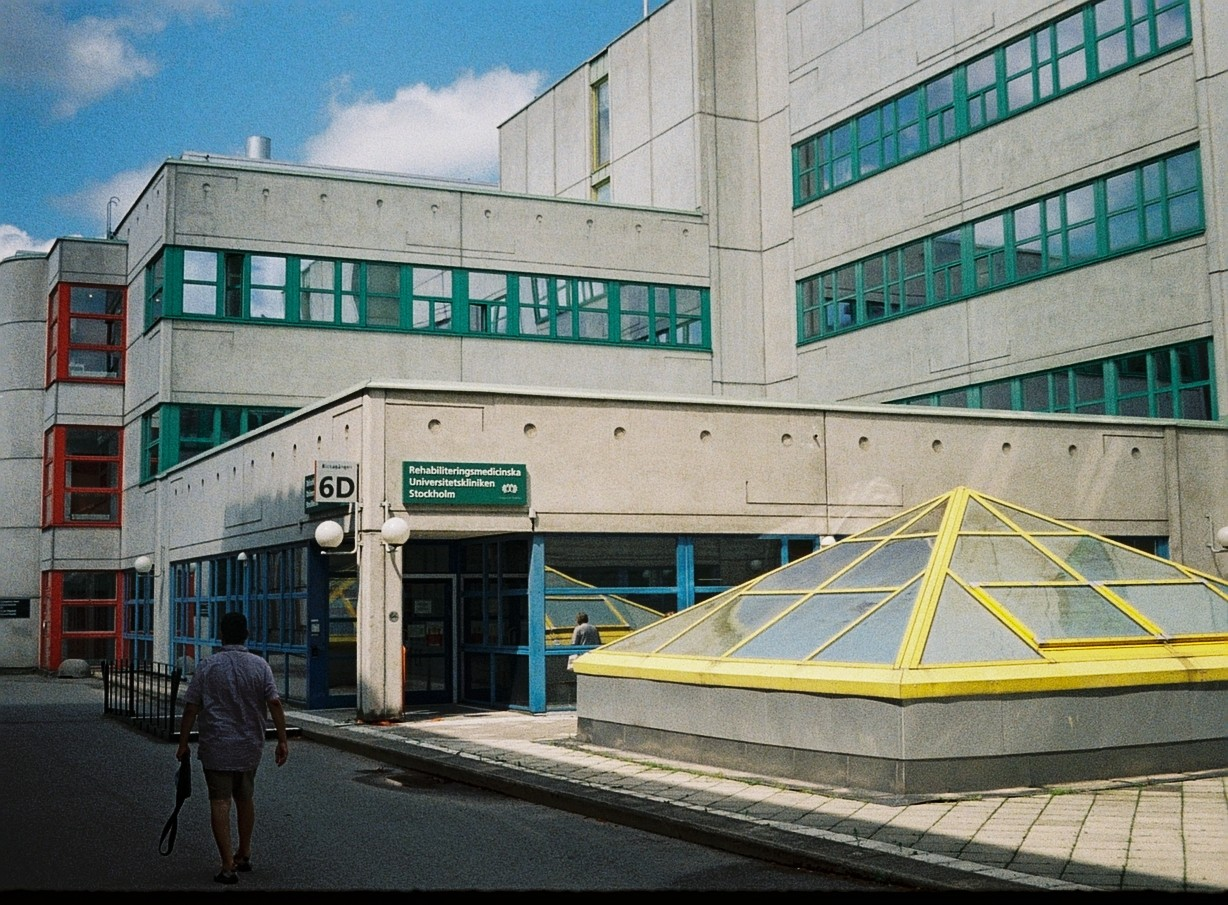
\includegraphics[keepaspectratio, width=0.83\textwidth]{innergaard2} \\

	\vspace*{-0.3mm}

	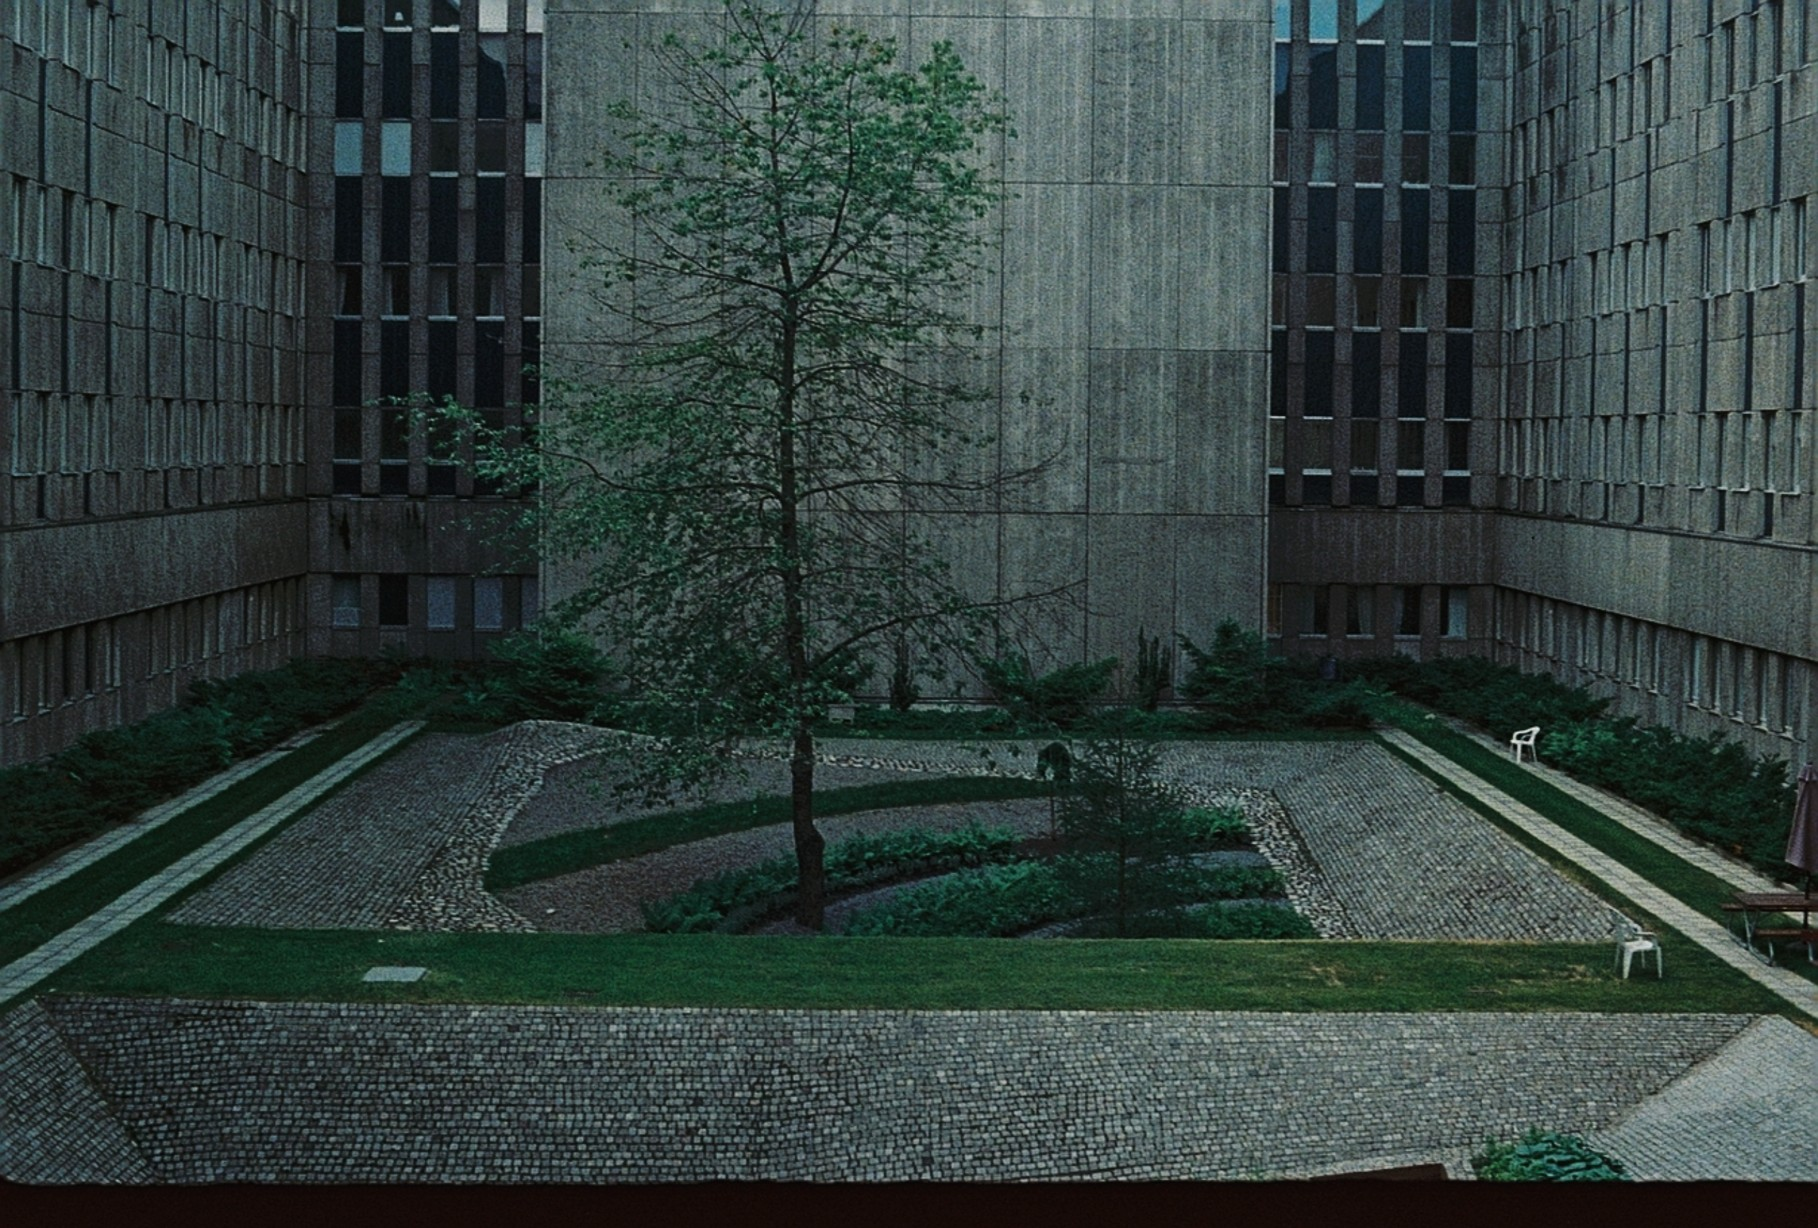
\includegraphics[keepaspectratio, width=0.83\textwidth]{innergaard1}
	\caption{Egna bilder tagna vid Huddinge sjukhus}
\end{figure}


% beskriv det cybernetiska - hur genom att förflytta fokus från teknologin till något extern så blev
% teknologin mer förkroppsligad.
Jag upplevde en förändring kring min relation till teknologi. Eftersom att jag använde mig av en extern,
utommusikalisk referensram var det lättare att använda tekniska verktyg. Det var som att ju mer jag hade
använt tekniken i sig själv som referensram för den musik jag skrev, desto mer otillgänglig och
svårgenomtränglig blev tekniken. Genom att ha fokuset på något externt blev även verktygen mer tillgängliga.
Genom att inte behandla tekniken som ett ideal i sig utan som ett hjälpmedel kunde jag inkorporera teknologin
i mig själv. Det var inte längre relationen mellan mig och teknologin som skulle utforskas, snarare relationen
mellan mig själv/teknologin och det externa.

\emph{Metamorfos}, det fjärde stycket jag presenterar i denna uppsats, kom ur ett mer tekniskt undersökande av
ljudfilers datastruktur, men jag har tagit med det med tanke på hur det arbetar med mellantillstånd. Dess
motor för ljudalstrande går ut på att låta ljudfiler övergå i varandra, en konstant transformation som inte
stannar upp. På ett sätt är det som att stycket har fastnat i ett liminalt tillstånd. Den existerar utan ett
före och ett efter, och ingen egentlig förlösning sker. I ett perfekt scenario kan den pågå för alltid, men i
praktiken har den bara spelat i högst 4 timmar utan att krascha. Dess ljudmaterial består av
telefoninspelningar av musikskisser från min sjukskrivning blandat med maskin- och naturljud från
sjukhusvistelser. Jag använde dem ursprungligen för att de var det senaste jag spelat in, men dess ursprung
bidrog till dess koppling till min egen association av det liminala. Ljuden jag har använt har en personlig
koppling men får även en intressant ljudande textur i och med styckets processering. Den har då både en
konkret och en abstrakt koppling till ett mellantillstånd, men den ena är en påtaglig ljudande effekt medan
den andra är en associativ effekt.

Jag lånar begreppet \emph{figurativiserande} från Delalande, men använder det för att beskriva en generativ
metod snarare än en analysmetod. Genom den här metoden har jag arbetat aktivt med att fundera över vilka
associationer som ljud kan ha, men oftast ur ett poiesiskt\footnote{Poiesis betyder att skapa och härstammar
ur det grekiska ordet för kreativitet. Motsatsen är \emph{estesis}, som kommer från ordet för att känna.
Orden används för att beskriva olika steg i en process, där det poietiska perspektivet är hur en avsändare
upplever sitt meddelande, medan det estetiska perspektivet är hur mottagaren upplever samma meddelande.}
perspektiv, utan en tanke på, eller snarare en önskan om att det inte skulle kunna kommuniceras genom musiken.
Jag tänkte att vissa figurativiseringar var för privata eller för banala för att jag skulle vara bekväm att
visa upp den delen av kompositionen. Styrkan med metoden var snarare att jag kunde luta mig mot
den, och att jag kunde vidareutveckla en komposition utifrån frågeställningen --\emph{"Hur förhåller sig mitt
ljudlandskap till ett associativt landskap?"}. Det är mellan dessa landskap som jag tänker att en gestalt
skulle förmedlas, en struktur som formats av min komposition men som skulle kunna tillåta ett mer associativt,
figurativt lyssnande hos åhöraren.


\pagebreak

% \phantomsection
% \addcontentsline{toc}{section}{Referenser}
\section{Referenser}
\phantomsection
\addcontentsline{toc}{subsection}{Litteratur}
\printbibliography[heading=subbibliography, title={Litteratur}, nottype=music, nottype=online, nottype=misc,
nottype=bilaga]
\pagebreak
\phantomsection
\addcontentsline{toc}{subsection}{Musik}
\printbibliography[heading=subbibliography, title={Musik}, type=music]
\phantomsection
\addcontentsline{toc}{subsection}{Uppslagsverk}
\printbibliography[heading=subbibliography, title={Uppslagsverk}, type=misc]
\phantomsection
\addcontentsline{toc}{subsection}{Webb}
\printbibliography[heading=subbibliography, title={Webb}, type=online]
\phantomsection
\addcontentsline{toc}{section}{6 \ \ Bilagor}
\printbibliography[heading=bibliography, title={Bilagor}, type=bilaga]
\includepdf[pages={6}]{./Framsidauppsats.pdf}
\end{document}
